

\actTitle{Worksheet 5.1}

\noindent \textbf{Instructions:}  Work together in groups of  3 or 4
to complete the following problems.\\

Student goals:
\begin{itemize}
\item State fundamental identities.
\item State the Pythagorean identitites.
\item Verify that a given expression is true.
  \begin{itemize}
  \item Using quotient identities
  \item Bringing together expressions using a common denominator.
  \item Factoring expressions.
  \item Using basic properties of trigonometric functions. (E.g.:
    $\sin(-\theta)=-\sin(\theta)$.
  \end{itemize}
\item Solve for values within expressions that involve logarithms.
\item Transform algebraic expressions by substituting trigonometric
  functions.
\end{itemize}

\vfill

\begin{enumerate}

\item Choose the sequence of steps below that verifies the identity,
  $$\tan(-x)\cos(x)=-\sin(x).$$
\begin{enumerate}
\item $\displaystyle \tan(-x)\cos(x)=-\tan(x)\cdot \cos(x)=-\frac{\cos(x)}{\sin(x)}\cdot \cos(x)=-\sin(x)$ \\ [1em]
\item $\displaystyle \tan(-x)\cos(x)=-\tan(x)\cdot \cos(x)=-\frac{\sin(x)}{\cos(x)}\cdot \cos(x)=-\sin(x)$  \\ [1em]
\item $\displaystyle \tan(-x)\cos(x)=\tan(x)\cdot -\cos(x)=\frac{\cos(x)}{\sin(x)}\cdot -\cos(x)=-\sin(x)$  \\ [1em]
\item $\displaystyle \tan(-x)\cos(x)=-\tan(x)\cdot -\cos(x)=-\frac{\sin(x)}{\cos(x)}\cdot -\cos(x)=-\sin(x)$  \\ [1em]
\end{enumerate}

\vfill
 
\clearpage

\item Verify each identity.
\begin{enumerate}

\item $\cot(-x)\sin(-x)=\cos(x)$

  \vfill

  
\item $\displaystyle \frac{\csc(x)-\sec(x)}{\csc(x)+\sec(x)}=\frac{\cot(x)-1}{\cot(x)+1}$

  \vfill
  \vfill

  \clearpage


\item $\displaystyle \frac{\tan(x)+\tan(y)}{\tan(x)\tan(y)-1}=\frac{\sin(x)\cos(y)+\cos(x)\sin(y)}{\sin(x)\sin(y)-\cos(x)\cos(y)}$


\vfill

\end{enumerate}



\clearpage

\item Choose the correct expression that completes the identity.
$$\sin^4(x)-\cos^4(x)=$$
\begin{enumerate}
\item $1-2\cos^2(x)$
\item $1+2\cos^2(x)$
\item $1-2\sin^2(x)$
\item $1+2\sin^2(x)$
\end{enumerate}
\vfill

\item Verify the identity.

\begin{enumerate}
\item $\left(6\cos(\theta)-\sin(\theta)\right)^2+\left(\cos(\theta)+6\sin(\theta)\right)^2=37$.
\vfill
\item $\displaystyle \frac{(\sin(x)+\cos(x))^2}{1+2\sin(x)\cos(x)}=1$
\vfill
\end{enumerate}

\clearpage

\item Choose the correct expression that completes the identity.
$$\frac{\cos^2(x)-\sin^2(x)}{1-\tan^2(x)}=$$
\begin{enumerate}
\item -1
\item 1
\item $\cos^2(x)$
\item $\sin^2(x)$
\end{enumerate}


\item Rewrite the expression in terms of the given function.
\begin{enumerate}
\item $\displaystyle \frac{\tan(x)+\cot(x)}{\sec(x)}$ in terms of $\csc(x)$
\vfill
\item $\displaystyle \frac{\tan(x)}{-1+\sec(x)}-\frac{\sec(x)}{\tan(x)}$ in terms of $\tan(x)$
\vfill

\end{enumerate}

\clearpage
\item Verify the identity.

\begin{enumerate}
\item $\tan^4(t)-\sec^4(t)=-2\tan^2(t)-1$
\vfill
\item $\displaystyle \csc(x)+\tan^2(x)\csc(x)=\frac{1}{\sin(x)\cos^2(x)}$
\vfill
\end{enumerate}


\end{enumerate}


\hwTitle{Section 5.1}

\begin{enumerate}
\item For each expression below make a substitution for $x$ where
  $x=\sin(\theta)$, $x=\sec(\theta)$, or $x=\tan(\theta)$ so that when
  the resulting expression is simplified there are no square roots.
  \begin{enumerate}
  \item ${\displaystyle \sqrt{1-x^2}}$
  \item ${\displaystyle \sqrt{1+x^2}}$
  \item ${\displaystyle \sqrt{x^2-1}}$
  \end{enumerate}
  How can you decide which substitution to use without trying each
  one?

\item For each expression below make a substitution for $x$ so that
  when simplified there are no square roots in the final expression.
  \begin{enumerate}
  \item ${\displaystyle \frac{\sqrt{9-x^2}}{x} }$
  \item ${\displaystyle x\sqrt{4+x^2}}$
  \item ${\displaystyle \frac{\sqrt{4x^2-1}}{x}}$
  \end{enumerate}

\item Use the diagram below to answer the following questions.

  \begin{tabular}{p{0.5\textwidth}p{0.5\textwidth}}
    
    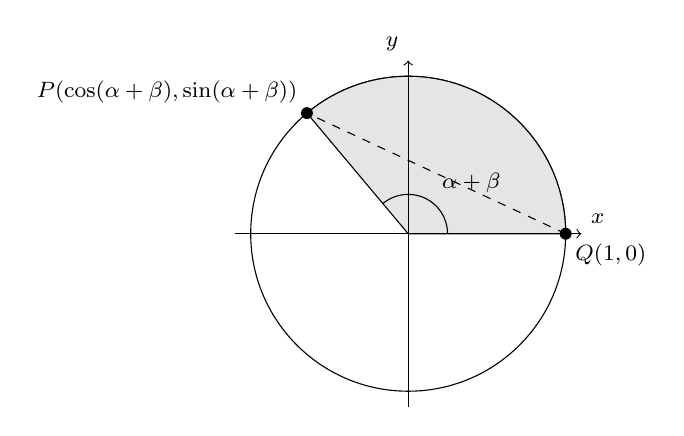
\begin{tikzpicture}[y=1cm, x=1cm,font=\sffamily]
      \draw[black] (0,0) circle (2);
      \draw[thin,black,fill=black!10!white] (0,0) -- (0:2) arc (0:130:2) -- (0,0);
      \draw[black,dashed] (0:2) -- (130:2);
      \draw[black] (0:0.5) arc (0:130:.5) node[pos=0.4,anchor=south west] {\footnotesize $\alpha+\beta$};
      \fill[black] (130:2) circle[radius=0.5ex] node[anchor=south east] {\footnotesize $ P(\cos(\alpha+\beta),\sin(\alpha+\beta))$};
      \fill[black] (0:2) circle[radius=0.5ex] node[anchor=north west] {\footnotesize $Q(1,0)$};
      \draw[thin,black,->] (-2.2,0.0) -- (2.2,0.0) node[anchor=south west] {\footnotesize $x$};
      \draw[thin,black,->] (0.0,-2.2) -- (0.0,2.2) node[anchor=south east] {\footnotesize $y$};
      % \node[black,anchor=south east] at (122:2) {$s$};
    \end{tikzpicture}

    &
      
    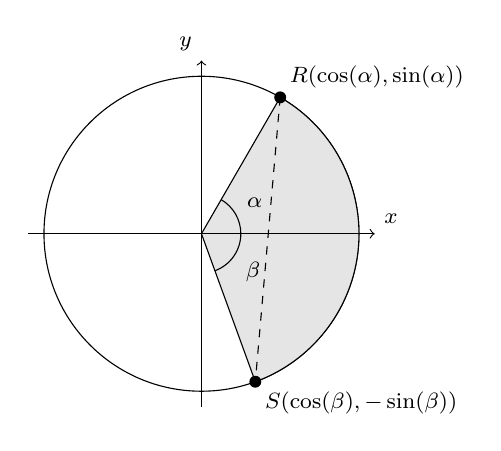
\begin{tikzpicture}[y=1cm, x=1cm,font=\sffamily]
      \draw[black] (0,0) circle (2);
      \draw[thin,black,fill=black!10!white] (0,0) -- (60:2) arc (60:-70:2) -- (0,0);
      \draw[black,dashed] (60:2) -- (-70:2);
      \draw[black] (0:0.5) arc (0:60:.5) node[pos=0.4,anchor=south west] {\footnotesize$\alpha$};
      \draw[black] (0:0.5) arc (0:-70:.5) node[pos=0.4,anchor=north west] {\footnotesize$\beta$};
      \fill[black] (60:2) circle[radius=0.5ex] node[anchor=south west] {\footnotesize $R(\cos(\alpha),\sin(\alpha))$};
      \fill[black] (-70:2) circle[radius=0.5ex] node[anchor=north west] {\footnotesize $S(\cos(\beta),-\sin(\beta))$};
      \draw[thin,black,->] (-2.2,0.0) -- (2.2,0.0) node[anchor=south west] {\footnotesize$x$};
      \draw[thin,black,->] (0.0,-2.2) -- (0.0,2.2) node[anchor=south east] {\footnotesize$y$};
      % \node[black,anchor=south east] at (122:2) {$s$};
    \end{tikzpicture}

  \end{tabular}

  \begin{enumerate}
  \item Verify that the distance squared between $P$ and $Q$ is $2-2\cos(\alpha+\beta)$.
  \item Verify that the distance squared between $R$ and $S$ is $2-2\cos(\alpha)\cos(\beta)+2\sin(\alpha)\sin(\beta)$.
  \item Why is the distance between $P$ and $Q$ the same as the distance between $R$ and $S$?
  \item What does this imply about an alternate way to express the
    value of $\cos(\alpha+\beta)$?
  \end{enumerate}
\end{enumerate}
